\chapter{Experimental Results}
\label{ch:result}
In this chapter we discuss about some experimental results 
of our analysis. We have developed a prototype model of heap 
dependence analysis at two levels: One at the intra-procedural 
level, which works for each procedure separately, and the other 
at the loop level, where the intra-procedural analysis is refined 
in the context of loop. The model is implemented in the Static 
Single Assignment (SSA) intermediate level of GCC (version 4.3.0)
\footnote{Available from http://gcc.gnu.org/}  
framework. The guideline for building and installing GCC from source, with 
newly added pass is given in Appendix A. 
We have conducted experiments over two example programs 
and two benchmark programs. 
The example programs are used to show how our loop-based 
approach successfully detects loop-carried dependences. These 
simple programs are based on single linked-list data structure 
presented in Figure~\ref{ch:loopdep}.3. Other benchmark programs 
\emph{TreeAdd} and \emph{Bisort} are 
drawn from Olden Suite. The prototype model, with manual 
intervention, successfully 
identifies the dependences present in benchmark programs

We have manually pre-processed the programs to be analysed, such that 
the heap accessing statements are normalized into binary statements. 
In the next step, based on type of heap access, the normalized 
statements are tagged accordingly. In the same step informations 
regarding pointers,  used and defined by the statement and the 
pointer field used to access the heap object are attached to 
each statement along with the access type. In the following sections 
we explain the experimental results for intra-procedural analysis 
and loop sensitive analysis.
%%%%%%%%%%%%%%%%%%%%%%%%%%%%%%%%%%%%%%%%%%%%%%%
\begin{figure}
  \begin{center}
    \scalebox{.85}{\begin{tabular}{ c | c }
     {\small \tt
      \begin{tabular}[b]{l}
		{\bf int} treeAdd(tree *t) \{     \\ 
		\ \ \ \ {\bf if} (t == NULL)           \\ 
		\ \ \ \ \ \ \ \ return 0;           \\ 
		\ \ \ \ tl = t$\rightarrow$left;    \\
        \ \ \ \ treeAdd(tl); \\
        \ \ \ \ tr = t$\rightarrow$right; \\
		\ \ \ \ treeAdd(tl); \\
		\ \ \ \ t$\rightarrow${num} = tl$\rightarrow${num} + tr$\rightarrow${num}; \\
		\}
      \end{tabular}
}	  
 %\cline{1-1}
    &
     {\tt
\begin{program}{0}
\UNL{0} int bisort(root,sprval,dir) 
% \FL\ \ldots
\UNL{1} HANDLE *root;
\UNL{1} int sprval, dir;
\UNL{0}\{
\UNL{1}	HANDLE *l;
\UNL{1}	HANDLE *r;
\UNL{1}	 l = root\rtarrow{left};
\UNL{1}      r = root\rtarrow{right};
\UNL{1}      val = root\rtarrow{value};
\UNL{1}     root\rtarrow{value}=bisort(l,val,dir);
\UNL{1}      ndir = !dir;
\UNL{1}      sprval=bisort(r,sprval,ndir);
\UNL{1}      sprval=bimerge(root,sprval,dir);
\UNL{1}    return sprval;
\UNL{0} \} 
  \end{program}
  }
 \\
%      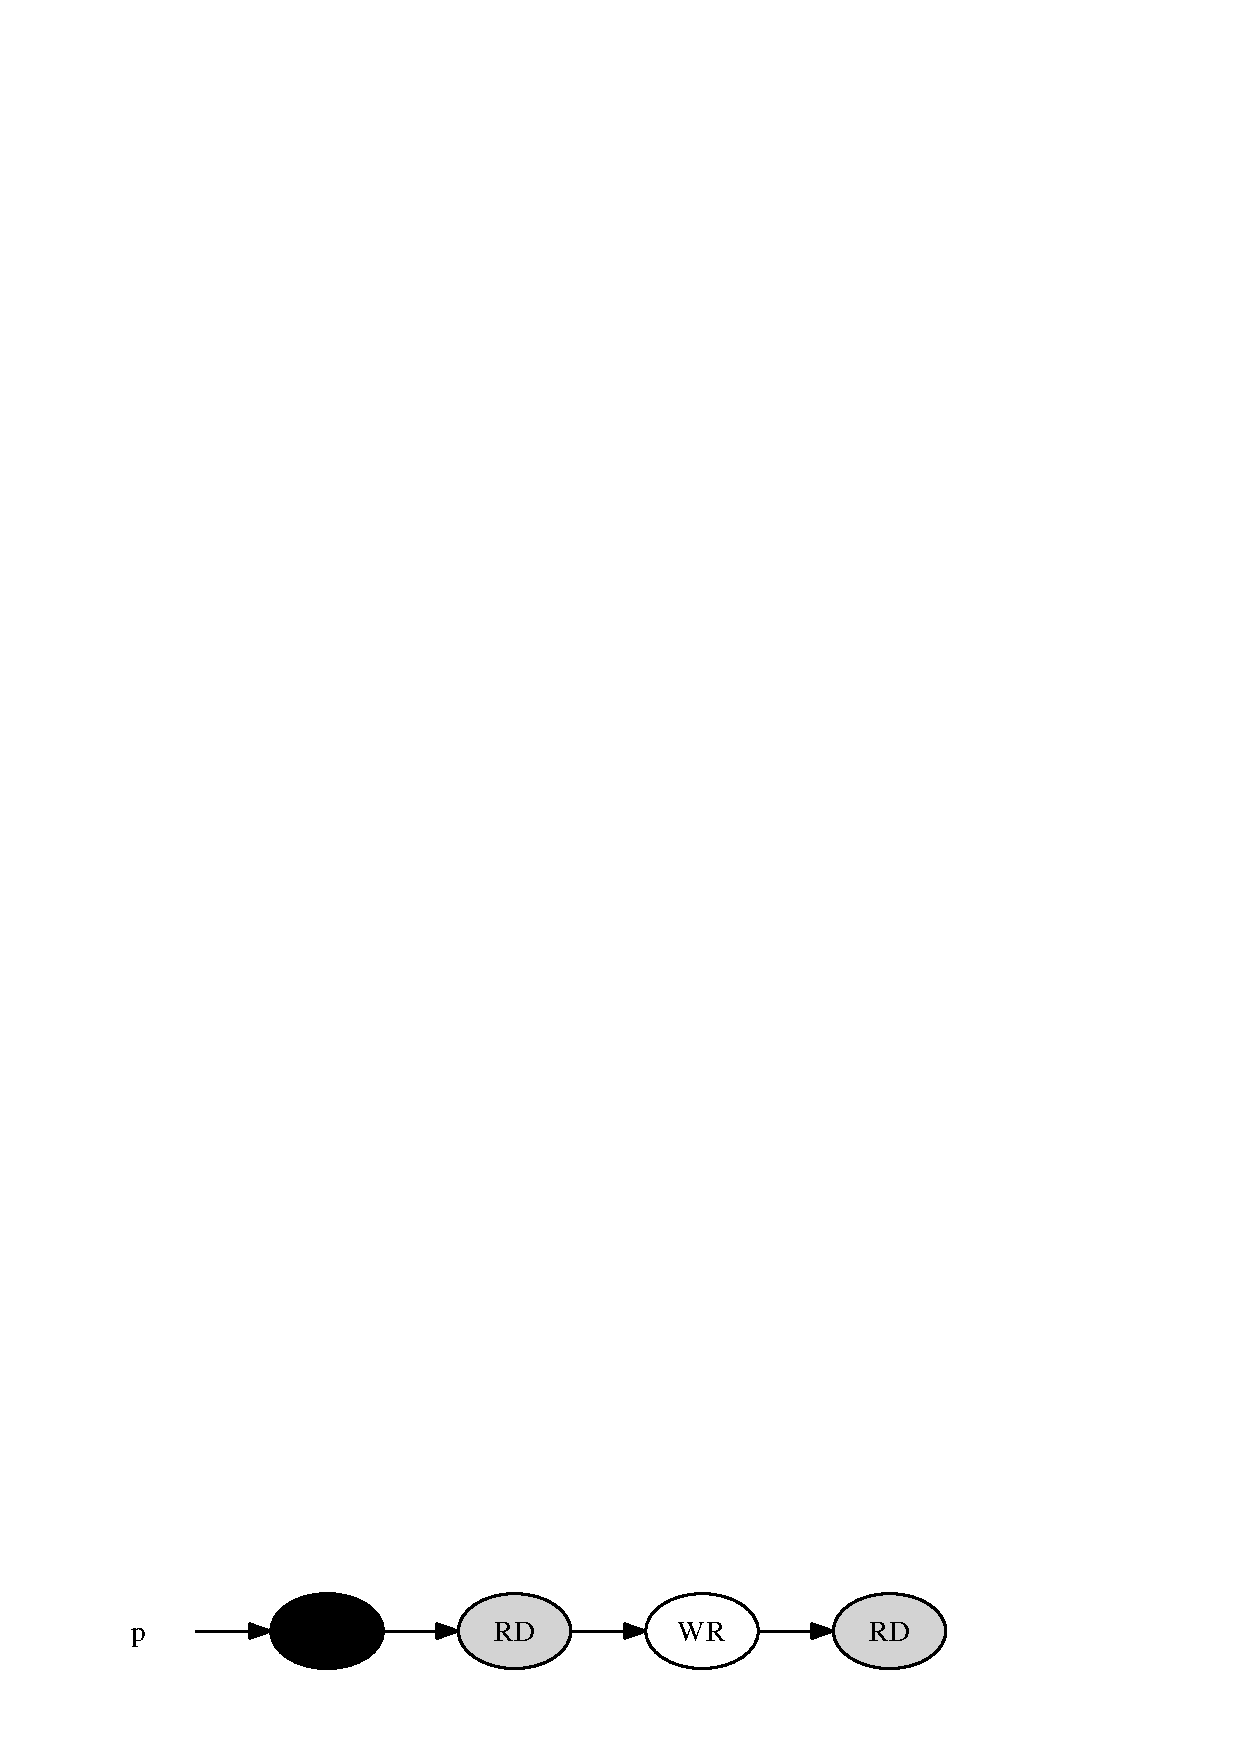
\includegraphics[scale=0.6]{grph_RD_WR} & \\
%     (a) & (b) \\
     (a) Function \emph{treeAdd} & 
      (b) Function \emph{bisort} \\
  \end{tabular}}
  \end{center}
  \hrule
  \caption{\label{fig:bench} Functions of benchmark programs}
%\hrule
\end{figure}
\begin{comment}
\begin{figure}
  \begin{center}
%    \scalebox{.85}{\begin{tabular}{ c c }
%     {\small \tt
      \begin{tabular}[b]{l}
		{\bf int} treeAdd(tree *t) \{     \\ 
		\ \ \ \ {\bf if} (t == NULL)           \\ 
		\ \ \ \ \ \ \ \ return 0;           \\ 
		\ \ \ \ tl = t$\rightarrow$left;    \\
        \ \ \ \ treeAdd(tl); \\
        \ \ \ \ tr = t$\rightarrow$right; \\
		\ \ \ \ treeAdd(tl); \\
		\ \ \ \ t$\rightarrow${num} = tl$\rightarrow${num} + tr$\rightarrow${num}; \\
		\}
      \end{tabular}
}	  
 %\cline{1-1}
%    &
     {\tt
\begin{program}{0}
\UNL{0} int bisort(root,sprval,dir) 
% \FL\ \ldots
\UNL{1} HANDLE *root;
\UNL{1} int sprval, dir;
\UNL{0}\{
\UNL{1}	HANDLE *l;
\UNL{1}	HANDLE *r;
\UNL{1}	 l = root\rtarrow{left};
\UNL{1}      r = root\rtarrow{right};
\UNL{1}      val = root\rtarrow{value};
\UNL{1}     root\rtarrow{value}=bisort(l,val,dir);
\UNL{1}      ndir = !dir;
\UNL{1}      sprval=bisort(r,sprval,ndir);
\UNL{1}      sprval=bimerge(root,sprval,dir);
\UNL{1}    return sprval;
\UNL{0} \} 
  \end{program}
  }
% \\
%      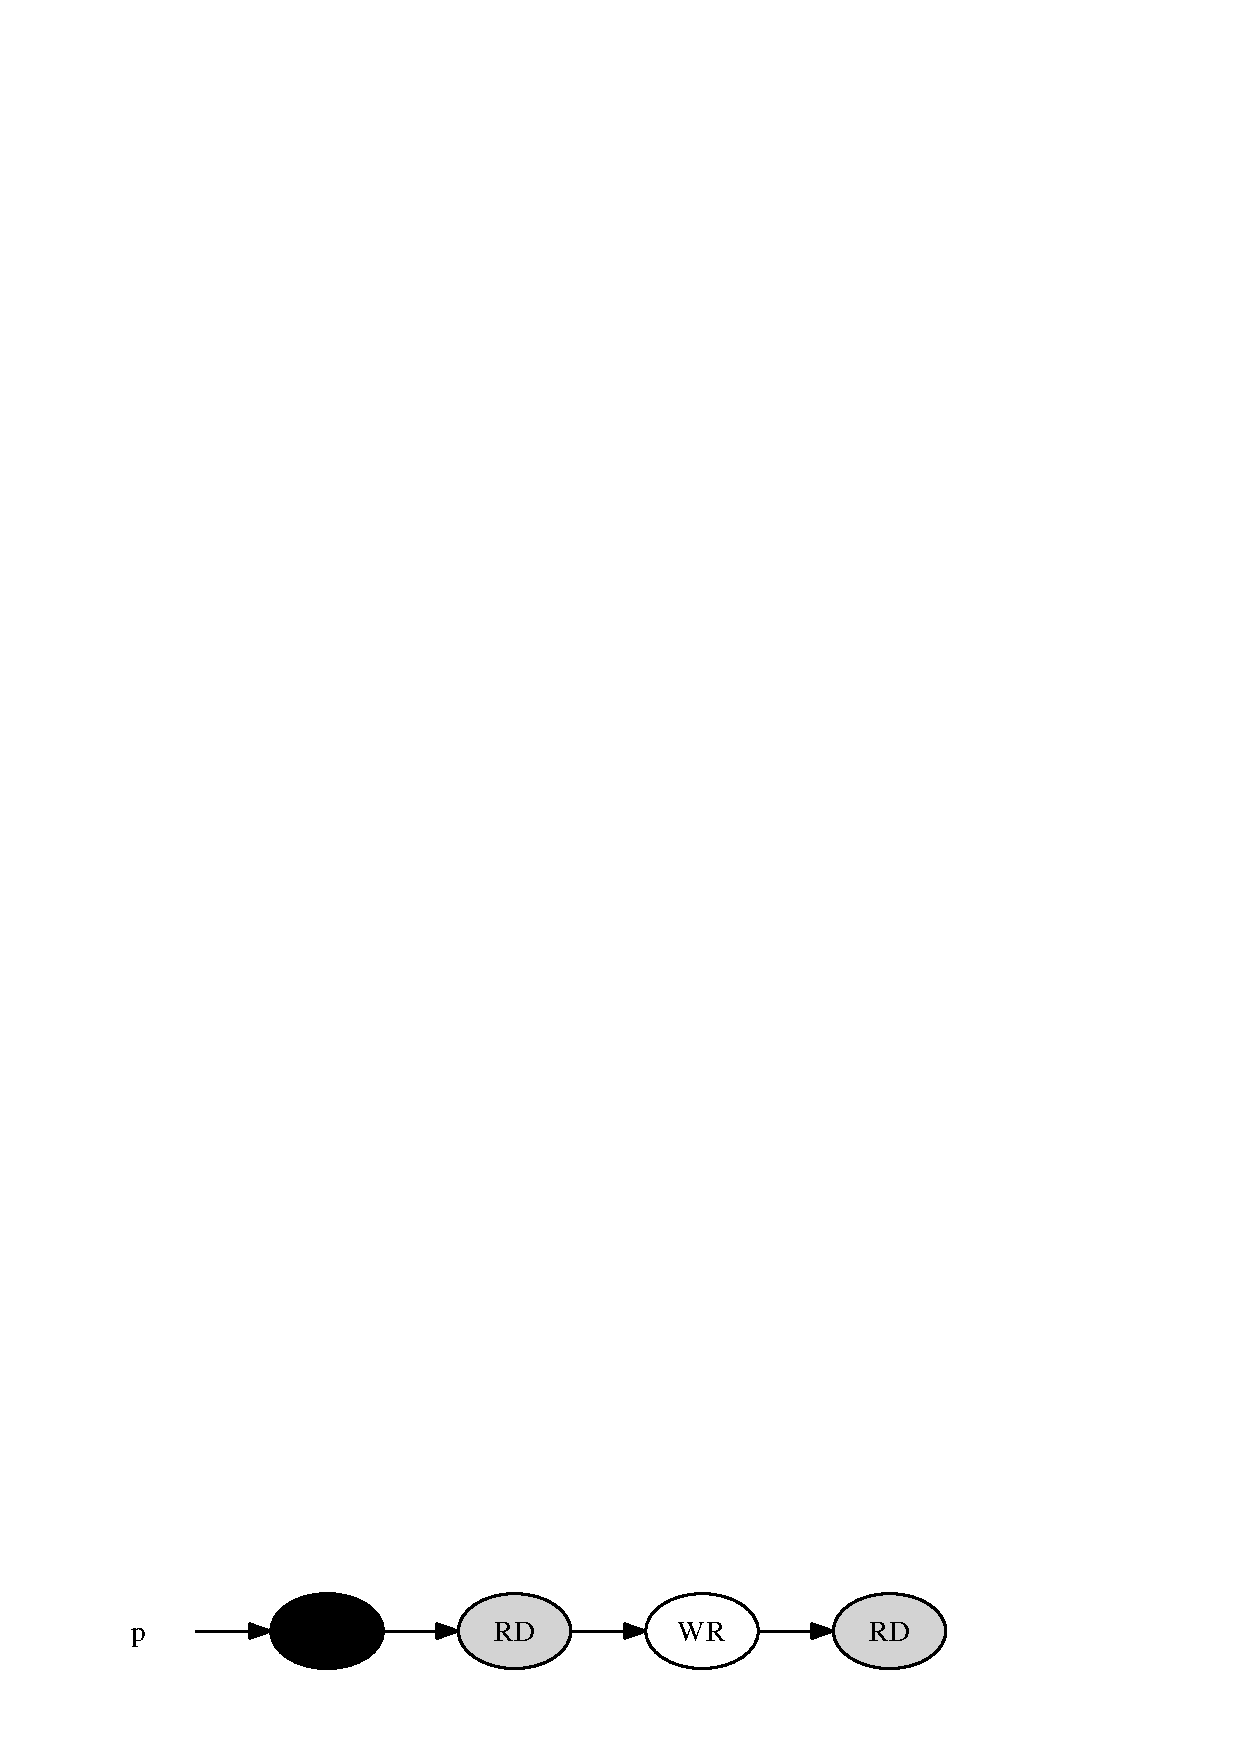
\includegraphics[scale=0.6]{grph_RD_WR} & \\
%      (a) & (b) \\
  %    (a) Nodes read and written by code & 
  %    (b) Code fragment traversing the data structure. \\
%   \end{tabular}}
  \end{center}
%  \hrule
  \caption{\label{fig:bisort} Function \emph{bisort}}
%\hrule
\end{figure}
\end{comment}
\section{Benchmarks}
Benchmark program \emph{TreeAdd} operates on binary tree and recursively adds the 
values of tree. The \emph{treeAdd} function from benchmark 
program \emph{TreeAdd} is analysed. This function  
recursively calls itself to compute values of its left and right subtrees. 
Left and right subtree values, thus computed are added to the value of the 
root to compute the value of whole tree. Figure~\ref{fig:bench}(a)  
shows the function \emph{treeAdd}. 
The main objective behind the analysis is to find out 
whether the recursive function calls on left and write subtrees 
can be executed in parallel. 
The function \emph{bisort} from the benchmark program \emph{Bisort} 
is also analysed to extract function call level parallelism. Function \emph{bisort} 
performs bitonic sort over binary tree by recursively calling itself on left and right subtrees 
of the root. 
The analysis is fine tuned in the context of loops. The experiments for loop sensitive 
dependence analysis are done on example programs \emph{List-1} and \emph{List-2} shown in 
Figure 5.3. Both the programs traverse single-linked list and in each iteration the functions  
read data from the current heap node and write the same data into the next node. But the function \emph{List-1} navigates iterations using two occurrences of pointer field \emph{next}, whereas,  function \emph{List-2} navigates using a single occurrence of \emph{next} pointer field. 
Hence by manual inspection it is clear that function \emph{List-1} does not have any loop  
dependence, but function \emph{List-2} poses loop dependences. 
%%%%%%%%%%%%%%%%%%%%%%%%%%%%%%%%%%%%%%%%%%%%%%%
\section{Results of Intra-Procedural Analysis}
The prototype model for intra-procedural dependence detection 
performs the state analysis which computes the set of pairs, consisting 
of pointer variable and path accessing corresponding symbolic heap location. 
In the next pass over the program, the model successfully computes 
the read and write sets of access paths for each heap accessing 
statement in the program. Next we manually check for each pair 
of heap accessing statements to find out any conflict in terms 
of data access. The interference predicate \ttf{isInterfering}, 
produced by shape analysis returns true if the access paths under 
objection lead to common heap location. 
%%%%%%%%%%%%%%%%%%%%%%%%%%%%%%%%
\begin{table}
\centering
\begin{tabular}{| l | c | c | c |}
\hline 
\bf{Program} & \bf{Traversal pattern} & \bf{Potential Dependence} & \bf{Type of dependence}\tn
\hline \hline
{\tt TreeAdd} & {\tt 2 nested} & {\tt No} & {\tt No dep.}\\
& {\tt rec. function} & & \\
\hline
{\tt Bisort} & {\tt 2 nested} & {\tt No} & {\tt No dep.}\\
& {\tt rec. function} & & \\
\hline
{\tt List-1} & {\tt single loop} & {\tt Yes} & {\tt Anti dep.}\\
\hline
{\tt List-2} & {\tt single loop} & {\tt Yes} & {\tt Anti dep.}\\
\hline
\end{tabular}
\caption{Result of programs tested by intra-procedural analysis} 
\label{fig:tableResutIntra}
%\hrule
\end{table}
%%%%%%%%%%%%%%%%%%%%%%%%%%%%%%%%%%%%%
In the Table~\ref{fig:tableResutIntra} we have given results of 
intra-procedural analysis. It reports no dependence at function 
call level for \emph{treeAdd} and \emph{bisort}. However, 
the analysis reports dependencies of type anti dependence for both  
example programs \emph{List-1} and \emph{List-2}.

%%%%%%%%%%%%%%%%%%%%%%%%%%%%%%%%%%%%%%%%%%%%%%%%%%%%%%%
\section{Results of Loop-Sensitive Analysis}
The basic prototype model identifies navigator variable and 
navigator expression, used by the loop to traverse over the 
data structure. It then computes the full length access paths 
being read or written by each statement within the body of the loop. 
The programs \emph{List-1} and \emph{List-2} are further analysed to refine dependence analysis. 
The previous analysis detects spurious dependencies in case of loop. 
Both example programs work on 
single linked list, which is of type Tree. As there exists no 
sharing within the underlying data structure, the generalized 
equations, formed by the access paths, are tested for loop-carried 
dependencies. Lamport test successfully reports no dependence for 
function \emph{List-1} and dependence of type 
anti dependence for function \emph{List-2}. 
\epsfig{file=certificate.ps,bbllx=0pt,bblly=0pt,bburx=594pt,bbury=842pt,width=10cm,angle=90}




